\documentclass[handout]{beamer} 
\title{ITCS 532:\\ 
6. Tractability and $p$-Time Reduction}
\date{}
\author{Rob Egrot}

\usepackage{amsmath, bbold, bussproofs,graphicx}
\usepackage{mathrsfs}
\usepackage{amsthm}
\usepackage{amssymb}
\usepackage[all]{xy}
\usepackage{multirow}
\usepackage{tikz-cd}

\newtheorem{exercise}[theorem]{Exercise}{\bfseries}{\upshape}


\newtheorem{proposition}[theorem]{Proposition}
\newcommand{\bN}{\mathbb{N}}
\newcommand{\bZ}{\mathbb{Z}}
\newcommand{\bQ}{\mathbb{Q}}
\newcommand{\bR}{\mathbb{R}}
\newcommand{\bP}{\mathbb{P}}
\newcommand{\tvs}{\textvisiblespace}
\newcommand{\ra}{\rightarrow}
\newcommand{\la}{\leftarrow}
\newcommand{\co}{\mathbf{code}}

\addtobeamertemplate{navigation symbols}{}{%
    \usebeamerfont{footline}%
    \usebeamercolor[fg]{footline}%
    \hspace{1em}%
    \insertframenumber/\inserttotalframenumber
}
\setbeamertemplate{theorems}[numbered]
\begin{document}

\begin{frame}
\titlepage
\end{frame}

\begin{frame}
\frametitle{Computational Complexity Theory}
\begin{itemize}
\item So far in this course we have only asked whether decision problems are decidable or semidecidable.
\vspace{0.2cm}
\item We only care about the existence, or provable non-existence, of algorithms.
\vspace{0.2cm}
\item We don't care how fast or slow they are.
\vspace{0.2cm}
\item E.g. Turing machines with multiple tapes are `equivalent' to standard Turing machines.
\vspace{0.2cm}
\item In the real world, it is important that algorithms run in a `reasonable amount of time'.
\vspace{0.2cm}
\item Here we start taking the running times of algorithms seriously.
\vspace{0.2cm}
\item This is the start of computational complexity theory. 
\end{itemize}
\end{frame}

\begin{frame}
\frametitle{Measuring Run Time - Computation Steps}
\begin{itemize}
\item We want our measure of the running time of an algorithm to be independent of the hardware we run it on. 
\vspace{0.2cm}
\item It might take my desktop several hours to run an algorithm that a supercomputer could run in a few seconds.
\vspace{0.2cm}
\item To solve this, we think about the number of steps involved in running the algorithm.
\vspace{0.2cm} 
\item We assume each computational step takes a constant amount of time on each system.
\vspace{0.2cm}
\item So in practice run time is a constant multiple of the number of steps (depending on computer power).
\vspace{0.2cm}
\item But the number of steps is the important thing for us. 
\vspace{0.2cm}
\item We can think of these steps as being steps in a Turing machine computation, or, more practically, CPU cycles.
\end{itemize}
\end{frame}

\begin{frame}
\frametitle{Measuring Run Time - Inputs}
\begin{itemize}
\item Another thing to consider is that we want our algorithms to run on \emph{inputs}.
\item So the time an algorithm takes will depend on the input we give it. 
\item I.e. Run time is a function of the input (strings over a finite alphabet). 
\item Usually impossible to describe this function exactly, so we think about the lengths of the inputs.
\item Different inputs of the same length may have different run times, so we ask about the \emph{worst case}.  
\item I.e. what is the slowest possible (halting) run time of this algorithm for an input of length $n$? 
\item This will give us a function of $n$, e.g. $f(n)=4n^3-5n +6$.
\item We ignore the cases where the computation does not halt.
\item We cannot usually define this function explicitly, so we think about bounds for it.
\end{itemize}
\end{frame}

\begin{frame}
\frametitle{Worst Case Analysis}
\begin{definition}[Big $O$ Notation]
Let $f$ and $g$ be functions from $\mathbb{R}$ to $\mathbb{R}$, and suppose $g(x)$ is strictly positive for large enough values of $x$ (i.e. after some point the values of $g(x)$ are all bigger than zero). We say $f=O(g)$ as $x\ra\infty$ if there are $x_0,c\in\mathbb{R}$ such that $|f(x)|\leq cg(x)$ for all $x\geq x_0$. 
\end{definition}
\begin{itemize}
\item We use big $O$ notation to roughly classify the worst case running times of algorithms. 
\item For example, if $f(n)=4n^3-5n +6$ then $f=O(n^3)$. 
\item Intuitively, for large $n$,  $f(n)$ is bounded above by $cn^3$. 
\item We are mainly interested in finding algorithms whose big $O$ worst case run time is as small as possible. 
\item In the real world we are often interested in the \emph{average case}. 
\item For example, \emph{Quicksort} has a worst case run time of $O(n^2)$, but the algorithm usually runs in $O(n\log(n))$. 
\end{itemize}
\end{frame}

\begin{frame}
\frametitle{Measuring Run Time - Growth Rate Comparison}
The following diagram (taken from the Wikipedia page for Big $O$ notation) illustrates the growth rates some common functions used in big $O$ notation. 
\[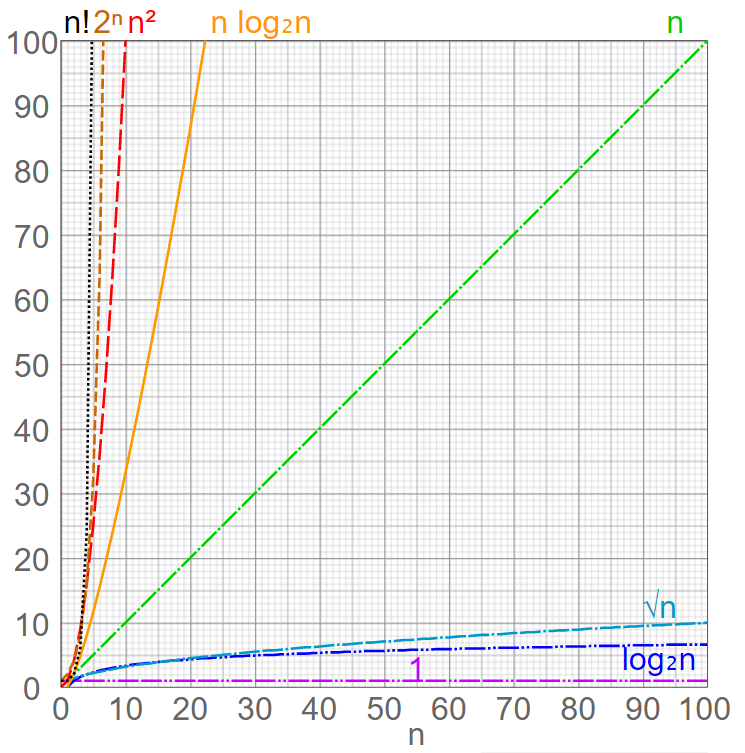
\includegraphics[width= 0.6\textwidth]{comp.png} \] 
\end{frame}

\begin{frame}
\frametitle{Algorithm Efficiency vs Computer Power}
\begin{itemize}
\item We want to understand why designing better algorithms for difficult problems is better than making faster computers (though faster computers are good too!).
\vspace{0.3cm}
\item Note that the `worst case analysis' here only applies to `large' values of $n$.
\vspace{0.3cm}
\item For small $n$ values the algorithm behaviour may be different.
\vspace{0.3cm}
\item We ignore this because small inputs are easy to deal with.
\vspace{0.3cm}
\item With inefficient algorithms, there is usually a limit point where input sizes become `too big'.
\vspace{0.3cm}
\item We ask how much increasing computer power increases this limit.
\end{itemize}
\end{frame}

\begin{frame}
\frametitle{Algorithm Efficiency vs Computer Power - Linear Case}
\begin{itemize}
\item Suppose we have an algorithm and we have computers $C_1$ and $C_2$ running this algorithm. 
\vspace{0.3cm}
\item $C_2$ is capable of performing $2^{12}$ computation steps in the time it takes $C_1$ to do 1.
\vspace{0.3cm}
\item So $C_2$ is 4096 times faster than $C_1$. 
\vspace{0.3cm}
\item In symbols $v_2 = 2^{12}v_1$. 
\vspace{0.3cm}
\item Suppose first that the algorithm runs in linear time ($O(n)$). 
\vspace{0.3cm}
\item What is the biggest input size machine $C_1$ can guarantee to handle in time $t$ (call this $n_1$)? 
\end{itemize}
\end{frame}

\begin{frame}
\frametitle{Algorithm Efficiency vs Computer Power - Linear Case}
\begin{itemize}
\item We have $f(n_1)\leq cn_1$ for some $c$.
\vspace{0.2cm} 
\item To guarantee that $C_1$ completes the computation in at most time $t$, we require that $cn_1\leq v_1t$.
\vspace{0.2cm} 
\item Rearranging the formula, we must have $n_1\leq \frac{v_1t}{c}$. 
\vspace{0.2cm} 
\item I.e., $n_1 =\lfloor \frac{v_1t}{c}\rfloor$. 
\vspace{0.2cm} 
\item What about $C_2$? 
\vspace{0.2cm} 
\item Remember that $v_2 = 2^{12}v_1$. 
\vspace{0.2cm} 
\item Similar to the case of $C_1$, we require $cn_2\leq v_2 t$, which rearranges to give $n_2\leq \frac{v_2t}{c}$. 
\vspace{0.2cm} 
\item I.e. $n_2=\lfloor \frac{2^{12}v_1t}{c}\rfloor \approx 2^{12}n_1$. 
\vspace{0.2cm} 
\item This is $2^{12}$ times bigger than for $C_1$, so is a huge improvement.
\end{itemize}
\end{frame}

\begin{frame}
\frametitle{Quadratic Case}
\begin{itemize}
\item Suppose now the algorithm runs in quadratic time.
\vspace{0.3cm}
\item I.e. $f(n)$ is $O(n^2)$, so $f(n)\leq cn^2$ for some constant $c$. 
\vspace{0.3cm}
\item Let $v_1$ and $v_2$ be as before. 
\vspace{0.3cm}
\item To guarantee completion in at most time $t$ by $C_1$ on an input of length $n_1$, we must have $cn_1^2\leq v_1t$. 
\vspace{0.3cm}
\item I.e. $n_1\leq \sqrt{\frac{v_1t}{c}}$.
\vspace{0.3cm} 
\item Similarly, for $C_2$, we must have input length \[n_2\leq \sqrt{\frac{v_2t}{c}}=\sqrt{\frac{2^{12}v_1t}{c}}= 2^6\sqrt{\frac{v_1t}{c}}.\]   
\item In other words, $n_2\approx 2^6n_1$.
\end{itemize}
\end{frame}

\begin{frame}
\frametitle{Exponential Case}
\begin{itemize}
\item Suppose now the algorithm that runs in exponential time.
\item  E.g. $f$ is $O(2^n)$. 
\item Then we have $2^{n_1}\leq \frac{v_1t}{c}$ and $2^{n_2}\leq \frac{v_2 t}{c}$ for some constant $c$. 
\item Taking logs base 2: 
\begin{itemize}
\item $n_1\leq \log(v_1) + \log(t) - \log (c)$. 
\item $n_2\leq \log(v_2) + \log(t) - \log (c)$.
\end{itemize}
\item Since $v_2=2^{12}v_1$, the second inequality can be rewritten as 
\begin{align*}n_2&\leq \log(2^{12}v_1) + \log(t) - \log (c)\\
&= \log(2^{12}) +\log(v_1) + \log(t) - \log (c)\\
&= 12 + \log(v_1) + \log(t) - \log (c).\end{align*}
\item I.e. $n_2\approx n_1 + 12$.
\item A very small improvement.
\end{itemize}
\end{frame}

\begin{frame}
\frametitle{Tractability and Intractability}
\begin{itemize}
\item Complexity theory divides algorithms into rough complexity classes based on their use of resources. 
\vspace{0.1cm}
\item The classes we discuss here are based on worst case run time. 
\vspace{0.1cm}
\item The difference between $O(n^2)$ and $O(n^3)$ can be very important in applications. 
\vspace{0.1cm}
\item For example, in some applications an $O(n^3)$ algorithm might be much too slow, but an $O(n^2)$ algorithm might be manageable. 
\vspace{0.1cm}
\item For some applications, e.g. in Big Data, $O(n^2)$ might be much too slow. 
\vspace{0.1cm}
\item Despite this, theorists often make a sharp distinction between  `efficient' and `inefficient' algorithms, and between `easy' and `hard' decision problems, based on the following definitions.
\end{itemize}
\end{frame}

\begin{frame}
\frametitle{Tractability and Intractability}
\begin{definition}[polynomial time]
An algorithm is polynomial time ($p$-time) if it is $O(n^k)$ for some $k\in\mathbb{N}$.
\end{definition}

\begin{definition}[tractable]
A decision problem is tractable if there is a polynomially time algorithm that decides it. It is \emph{intractable} otherwise. 
\end{definition}
\begin{itemize}
\item As an approximation, complexity theorists consider tractable problems to be `easy', and intractable ones to be `hard'. 
\item In practice, a polynomial time algorithm might be much too slow for practical use, as mentioned before. 
\item Of course, finding a polynomial time algorithm for a problem, thus demonstrating its `easiness', may not be easy at all!
\end{itemize}
\end{frame}

\begin{frame}[fragile]
\frametitle{The simple PRIME Algorithm}
Consider the following algorithm:
\begin{verbatim}
Prime(n).
answer = `true'
for i = 2 to n-1
	if i divides n then answer = `false'
return answer.	
\end{verbatim} 

\end{frame}

\begin{frame}
\frametitle{The Run Time of PRIME}
\begin{itemize}
\item Say we have an $O(n^2)$ algorithm to test if $i$ divides $n$. 
\item Worst case run time of `Prime' is $O(n^3)$. 
\item But to run this on a TM we need to encode natural numbers using a finite alphabet.
\item Length of the input is the number of symbols used.
\item E.g. a binary number of length $n$ can represent a natural number up to $2^n-1$. 
\item So considered as a function of binary input length this algorithm has a worst case run time of $O((2^n)^3)=O(2^{3n})$.
\item But if we use unary notation then the algorithm does run in $p$-time in length of input. 
\item So there is a relationship between how we encode problems and the running times of algorithms we can use to solve them. 
\item We can make algorithms look more efficient by encoding the problem in an inefficient way.
\end{itemize}
\end{frame}

\begin{frame}
\frametitle{Polynomial Time Reduction}
\begin{itemize}
\item Previously we saw how we can order decision problems in terms of their decidability using reduction. 
\vspace{0.2cm}
\item That is, $A\leq B$ if there's an algorithm that turns `yes' instances of $A$ into `yes' instances of $B$, and `no' instances of $A$ into `no' instances of $B$. 
\vspace{0.2cm}
\item I.e. problem $B$ is `at least as hard' as problem $A$.
\vspace{0.2cm}
\item We can extend the idea of reduction to order decision problems in terms of their polynomial time solvability. 
\vspace{0.2cm}
\item We write $A\leq_p B$ if there is a $p$-time algorithm that reduces $A$ to $B$. 
\vspace{0.2cm}
\item Then, if we had a $p$-time algorithm for solving $B$ we could combine it with the $p$-time conversion algorithm to get a $p$-time algorithm for solving $A$.
\end{itemize}
\end{frame}

\begin{frame}
\frametitle{Polynomial Time Reduction}
\begin{itemize}
\item Actually there is a complication here. 
\item Our first algorithm converts instances of $A$ to instances of $B$ in $p$-time, and the second algorithm solves $B$ in $p$-time. 
\item But the second algorithm runs in $p$-time on the size of its input, and the algorithm that converts instances of $A$ to instances of $B$ does not necessarily preserve their sizes. 
\item Could the converted input be more than polynomial in the length of the original?
\item No, because the fact that the conversion algorithm is $p$-time bounds the size of the converted instance. 
\item I.e. if the conversion algorithm runs in time $n^k$ and the original $A$ instance has size $m$, then the converted instance can be at most size $cm^k$ (constant $c$). 
\item If the algorithm for solving $B$ is $O(n^l)$, the worst case run time for the combined algorithm is $O((n^k)^l)=O(n^{kl})$.  
\end{itemize}
\end{frame}

\begin{frame}
\frametitle{Properties of $\leq_p$}
\begin{theorem}
$\leq_p$ is transitive.
\end{theorem}
\begin{proof}
\begin{itemize}
\item Suppose $A\leq_p B$ and $B\leq_p C$. 
\item If $I$ is an instance of $A$ let $f(I)$ be the result of applying the reduction of $A$ to $B$ to $I$. 
\item If $J$ is an instance of $B$ let $g(J)$ be the result of applying the reduction of $B$ to $C$ to $J$. 
\item $g(f(I))$ is a reduction of $A$ to $C$. 
\item We need to check $g\circ f$ is $p$-time. 
\item Suppose the reduction of $A$ to $B$ is $O(n^k)$ for some $k$, and the reduction from $B$ to $C$ is $O(n^l)$ for some $l$. 
\item Then the maximum size of $f(I)$ is $O(n^k)$, so $g\circ f$ is $O((n^k)^l)=O(n^{kl})$.
\end{itemize}
\end{proof}
\end{frame}

\begin{frame}
\frametitle{Properties of $\leq_p$}
\begin{exercise}
Why is it obvious that $\leq_p$ is reflexive?
\end{exercise}

\begin{theorem}\label{T:Pmin}
Let $A$ and $B$ be decision problems. Then, if there is a $p$-time algorithm for solving $A$, and if $B$ has at least one `yes' instance and at least one `no' instance, then $A\leq_p B$.
\end{theorem}
\begin{proof}
\begin{itemize}
\item There's a $p$-time algorithm for solving $A$, by assumption. 
\item Just use this algorithm to check if they are `yes' or `no' instances of $A$ then convert them to either the `yes' or `no' instance of $B$ appropriately. 
\item This `conversion' is constant time,  as we always convert to either the fixed `yes' instance, or the fixed `no' instance.
\end{itemize} 
\end{proof}
\end{frame}

\begin{frame}
\frametitle{$P$-Time Equivalence}
\begin{itemize}
\item We know that $\leq_p$ is not symmetric. 
\item Because if $\leq_p$ were symmetric it would follow from theorem \ref{T:Pmin} that every decision problem would have a $p$-time solution. 
\item Since there are problems that are not even decidable this is impossible. 
\item However, we can use $\leq_p$ to define a relation between decision problems that is reflexive, transitive, and symmetric (i.e. an equivalence relation).
\end{itemize} 
\begin{definition}[$\equiv_p$]
Decision problems $A$ and $B$ are \emph{$p$-time equivalent} if $A\leq_p B$ and $B\leq_p A$.
\end{definition} 

\end{frame}

\begin{frame}
\frametitle{The Hamiltonian Circuit Problem}
\begin{definition}[Hamiltonian circuit] 
Given a finite simple graph $G$ with $n$ vertices, a Hamiltonian circuit is a sequence $c=(v_1,v_2,\ldots,v_n)$ such that
\begin{enumerate}
\item if $v_i$ and $v_j$ occur consecutively in the sequence then there is an edge from $v_i$ to  $v_j$ in $G$,
\item every vertex of $G$ occurs in $c$, and
\item there is an edge from $v_n$ to $v_1$.  
\end{enumerate}  
\end{definition}
Informally a Hamiltonian circuit is a path in $G$ that passes through every vertex exactly once before returning to its origin.
\begin{definition}[$HCP$]
The Hamiltonian circuit problem ($HCP$) is whether a given finite undirected simple graph has a Hamiltonian circuit.
\end{definition}

\end{frame}

\begin{frame}
\frametitle{The Travelling Salesman Decision Problem}
\begin{definition}[weighted graph]
A weighted graph is a graph where every edge is associated with a number (usually a non-negative integer). This number can be thought of as the `cost' of traveling along that edge.
\end{definition}

\begin{definition}[$TSDP$]
The traveling salesman decision problem ($TSDP$) has instances $(G,d)$, where $G$ is a finite complete undirected weighted simple graph with non-negative integer weights, and $d$ is a non-negative integer. The question is whether there is a Hamiltonian circuit in $G$ such that the sum of the weights of the edges used in the circuit is less than or equal to $d$. 
\end{definition}

\end{frame}

\begin{frame}
\frametitle{$HCP\leq_p TSDP$}
\begin{theorem}
$HCP\leq_p TSDP$, ($p$-time in the number of vertices plus the number of edges of the graph $G$).
\end{theorem}
\textbf{Proof}
\begin{itemize}
\item An instance of $HCP$ is a finite undirected simple graph $G$ with $n$ vertices and $e$ edges. 
\item We will convert $G$ into a pair $(G',d)$ where $G'$ is a finite complete undirected weighted simple graph, and $d$ is a non-negative integer. 
\item This is an instance of $TSDP$. 
\item We then show that `yes' instance of $HCP$ become `yes' instances of $TSDP$, and similar for `no' instances. 
\item Finally we check that the conversion algorithm runs in $p$-time as a function of $n+e$.
\end{itemize} 

\end{frame}

\begin{frame}
\frametitle{$HCP\leq_p TSDP$ - The Reduction}
\begin{itemize}
\item Let $G'$ have the same vertices as $G$. 
\vspace{0.3cm}
\item To be an instance of $TSDP$ $G'$ must be complete, so we add edges for each pair of vertices.
\vspace{0.3cm}
\item In $G'$, edges from $G$ get weight 0, new edges have weight $1$. 
\vspace{0.3cm}
\item We set $d=0$. 
\vspace{0.3cm}
\item So $G'$ has a Hamiltonian circuit with total weight 0 if and only if there is a Hamiltonian circuit in $G$. 
\end{itemize} 
\end{frame}

\begin{frame}
\frametitle{$HCP\leq_p TSDP$ - How Fast is the Reduction?}
\begin{itemize}
\item The reduction is correct, but how fast is it?.
\vspace{0.3cm}
\item We have to clone the vertices of $G$. This is $O(|V|)$. 
\vspace{0.3cm}
\item Then we add edges for pairs of vertices. There are $n \choose 2$ pairs of vertices of $G$, so this is $O(|V|^2)$. 
\vspace{0.3cm}
\item Setting the weights involves checking every edge of $G'$ to see if it corresponds to an edge of $G$. 
\vspace{0.3cm}
\item Can check every edge of $G$ to see if it is an edge between $v$ and $v'$ for every pair $v,v'\in V$. 
\vspace{0.3cm}
\item This is $O(|E|\times|V|^2)$.
\vspace{0.3cm}
\item Setting $d=0$ is a constant time operation, say $c$. So the whole process takes $O(|V|)+O(|V|^2)+O(|E|\times|V|^2)+c$, which is $O((|V|+|E|)^3)$ at most.
\end{itemize} 
\end{frame}

\begin{frame}
\frametitle{$TSDP\leq_p HCP$}
\begin{itemize}
\item The converse to the theorem we just proved is also true. 
\vspace{0.5cm}
\item If you are feeling ambitious you can try to prove it directly using $p$-time reduction. 
\vspace{0.5cm}
\item This is a lot harder than the direction proved in the theorem. 
\vspace{0.5cm}
\item We will prove it using some powerful general theory at the end of the course.
\end{itemize}
\end{frame}

\end{document}